\let\negmpace\undefined
\let\negthickspace\undefined
\documentclass[journal]{IEEEtran}
\usepackage[a5paper, margin=10mm, onecolumn]{geometry}
%\usepackage{lmodern} % Ensure lmodern is loaded for pdflatex
\usepackage{tfrupee} % Include tfrupee package
\setlength{\headheight}{1cm} % Set the height of the header box
\setlength{\headsep}{0mm}     % Set the distance between the header box and the top of the text
\usepackage{gvv-book}
\usepackage{gvv}
\usepackage{cite}
\usepackage{amsmath,amssymb,amsfonts,amsthm}
\usepackage{algorithmic}
\usepackage{graphicx}
\usepackage{textcomp}
\usepackage{xcolor}
\usepackage{txfonts}
\usepackage{listings}
\usepackage{enumitem}
\usepackage{mathtools}
\usepackage{gensymb}
\usepackage{comment}
\usepackage[breaklinks=true]{hyperref}
\usepackage{tkz-euclide} 
\usepackage{listings}
% \usepackage{gvv}                                        
\def\inputGnumericTable{}                                 
\usepackage[latin1]{inputenc}                                
\usepackage{color}                                            
\usepackage{array}                                            
\usepackage{longtable}                                       
\usepackage{calc}                                             
\usepackage{multirow}                                         
\usepackage{hhline}                                           
\usepackage{ifthen}                                           
\usepackage{lscape}
\renewcommand{\thefigure}{\theenumi}
\renewcommand{\thetable}{\theenumi}
\setlength{\intextsep}{10pt} % Space between text and floats
\numberwithin{equation}{enumi}
\numberwithin{figure}{enumi}
\renewcommand{\thetable}{\theenumi}
\title{Assignment4}
\author{Teja Vardhan Shannu}
\date{August 2024}

\begin{document}
\maketitle

\section*{Question}
Given the vertices of a triangle \( PQR \) as P$\brak{2,2}$, Q$\brak{-4,-4}$, and R$\brak{5,-8}$, find the length of the median through \( R \).

\section*{Solution}


\begin{table}[h!]

\centering    

\begin{tabular}{|c|c|}
\hline

Input & Output \\
\hline
P & {P} = $\begin{pmatrix} 2 \\ 2 \end{pmatrix}$ \\
Q & {Q} = $\begin{pmatrix} -4 \\ -4 \end{pmatrix}$\\
R & {R} = $\begin{pmatrix} 5 \\ -8 \end{pmatrix} $\\
M & Midpoint of P,Q    \\

\hline
\end{tabular}
\end{table}







The midpoint \( M \) of the line segment \( PQ \) is calculated as:



\begin{align*}
 M &= \frac{P + Q}{2} \\
\mathbf{R} &= \begin{pmatrix} 5 \\ -8 \end{pmatrix}, \quad \mathbf{M} = \begin{pmatrix} -1 \\ -1 \end{pmatrix} \\
\mathbf{RM} &= \mathbf{R} - \mathbf{M} = \begin{pmatrix} 5 \\ -8 \end{pmatrix} - \begin{pmatrix} -1 \\ -1 \end{pmatrix} \\
&= \begin{pmatrix} 5 - (-1) \\ -8 - (-1) \end{pmatrix} = \begin{pmatrix} 6 \\ -7 \end{pmatrix}
\end{align*}




\[
\| \mathbf{RM} \|_2 = \sqrt{\mathbf{(RM)
}^T \mathbf{RM}} = \sqrt{\begin{bmatrix} 6 & -7 \end{bmatrix} \begin{bmatrix} 6 \\ -7 \end{bmatrix}} = \sqrt{6^2 + (-7)^2} = \sqrt{85}
\]





\begin{figure}[h!]
  \hspace{-1cm}
  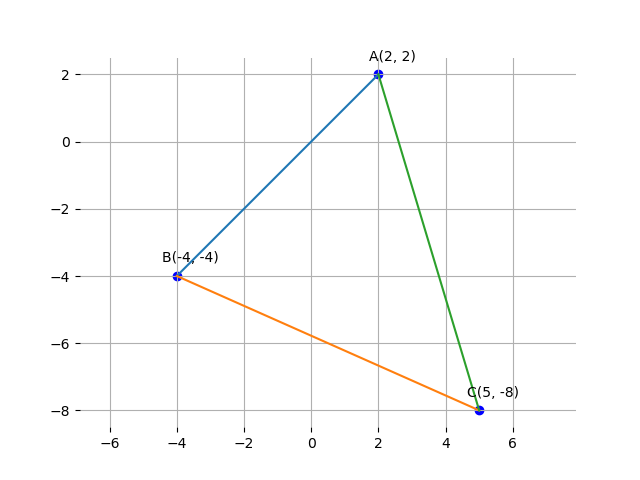
\includegraphics[width=1.2\textwidth]{Figure_1.png}
  
  \caption{The plot of the points }
  \label{fig:your_label}
\end{figure}




\end{document}

